\documentclass[a4paper, 12pt]{article} % тип документа

%%%Библиотеки
    %\usepackage[warn]{mathtext}	
    \usepackage[T2A]{fontenc}   %Кодировка
    \usepackage[utf8]{inputenc} %Кодировка исходного текста
    \usepackage[english, russian]{babel} %Локализация и переносы
    \usepackage{caption}
    \usepackage{gensymb}
    %\usepackage{listings}
    \usepackage{amsmath, amsfonts, amssymb, amsthm, mathtools}
    %\usepackage[warn]{mathtext}
    %\usepackage[mathscr]{eucal}
    %\usepackage{wasysym}
    %\usepackage{graphicx} %Вставка картинок правильная
    %\usepackage{pgfplots}
    \usepackage{indentfirst}
    %\usepackage{float}    %Плавающие картинки
    %\usepackage{wrapfig}  %Обтекание фигур (таблиц, картинок и прочего)
    \usepackage{fancyhdr} %Загрузим пакет
    %\usepackage{lscape}
    %\usepackage{xcolor}
    %\usepackage[normalem]{ulem}
    
    \usepackage{titlesec}
    \titlelabel{\thetitle.\quad}

    \usepackage{hyperref}

%%%Конец библиотек

%%%Настройка ссылок
    \hypersetup
    {
        colorlinks = true,
        linkcolor  = blue,
        filecolor  = magenta,
        urlcolor   = blue
    }
%%%Конец настройки ссылок


%%%Настройка колонтитулы
    \pagestyle{fancy}
    \fancyhead{}
    \fancyhead[L]{1.4.5}
    \fancyhead[R]{Глаз Роман, группа Б01-007}
    \fancyfoot[C]{\thepage}
%%%конец настройки колонтитулы



\begin{document}
                        %%%%Начало документа%%%%


%%%Начало титульника
\begin{titlepage}

    \newpage
    \begin{center}
        \normalsize Московский физико-технический институт \\(госудраственный университет)
    \end{center}

    \vspace{6em}

    \begin{center}
        \Large Лабораторная работа по общему курсу физики\\Термодинамика и молекулярная физика
    \end{center}

    \vspace{1em}

    \begin{center}
        \Large \textbf{1.4.5. Изучение колебаний струны}
    \end{center}

    \vspace{2em}

    \begin{center}
        \large Глаз Роман Сергеевич\\
        Группа Б01-007
    \end{center}

    \vspace{\fill}

    \begin{center}
        Долгопрудный \\2021
    \end{center}
    
\end{titlepage}
%%%Конец Титульника


%%%Настройка оглавления и нумерации страниц
    \thispagestyle{empty}
    \newpage
    \tableofcontents
    \newpage
    \setcounter{page}{1}
%%%Настройка оглавления и нумерации страниц


                    %%%%%%Начало работы с текстом%%%%%%


\textbf{Цель работы:}  изучение поперечных стоячих волн на струне; определение собственных частот колебаний струны; исследование зависимости скорости распространения
поперечных волн на струне в зависимости от её натяжения.\\

\textbf{Используемое оборудование:} закрепленная на станине стальная струна, набор грузов,
электромагнитные датчики, звуковой генератор, двухканальный осциллограф, частотомер.

\section{Теоретические сведения о струне и колебаниях}

Струной в акустике называют однородную тонкую гибкую упругую нить. Примерами могут служить сильно натянутый шнур или трос, струны гитары, скрипки и других музыкальных инструментов. В данной работе изучаются поперечные колебания стальной гитарной струны, натянутой горизонтально и закрепленной между двумя неподвижными зажимами.

Основное свойство струны — гибкость — обусловлено тем, что её поперечные размеры малы по сравнению с длиной. Это означает, что напряжение
в струне может быть направлено только вдоль неё, и позволяет не учитывать
изгибные напряжения, которые могли бы возникать при поперечных деформациях (то есть, при изгибе струны).

В натянутой струне возникает поперечная упругость, т.е. способность сопротивляться всякому изменению формы, происходящему без изменения
объема. При вертикальном смещении произвольного элемента струны, возникают силы, действующие на соседние элементы, и в результате вся струна
приходит в движение в вертикальной плоскости, т.е. возбуждение «бежит» по
струне. Передача возбуждения представляет собой поперечные бегущие
волны, распространяющиеся с некоторой скоростью в обе стороны от места
возбуждения. В ненатянутом состоянии струна не обладает свойством поперечной упругости и поперечные волны на ней невозможны.

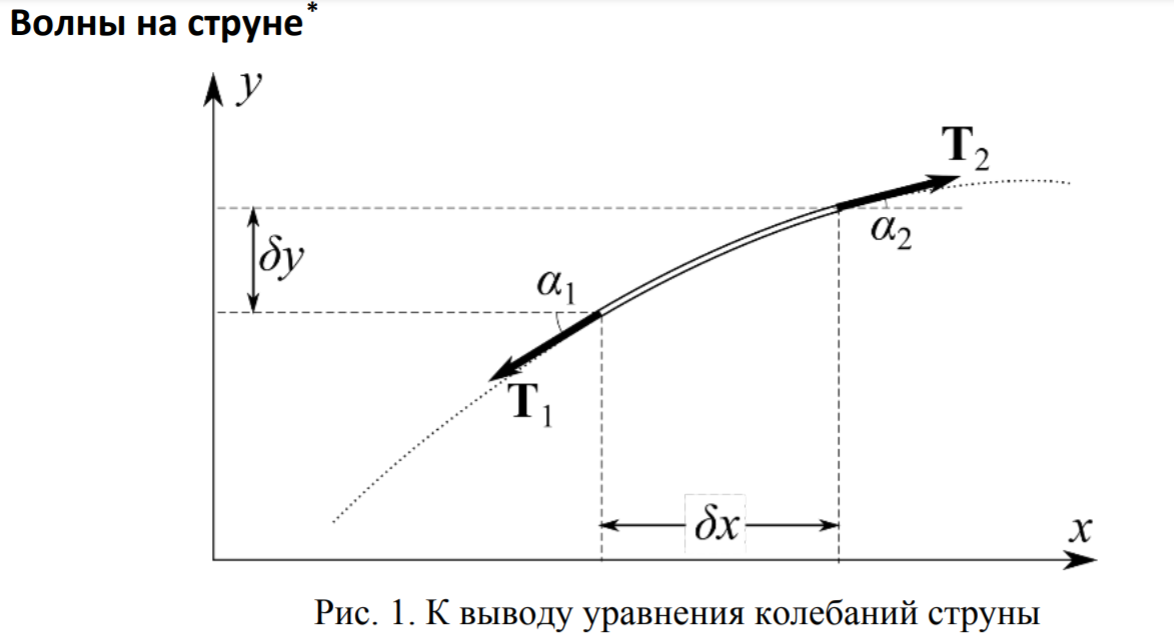
\includegraphics[width=\textwidth]{1.4.5 1}

Рассмотрим гибкую однородную струну, в которой создано натяжение $T$,
и получим дифференциальное уравнение, описывающее её малые поперечные свободные колебания. Отметим, что если струна расположена горизонтально в поле тяжести, величина $T$ должна быть достаточна для того, чтобы в
состоянии равновесия струна не провисала, т. е. сила натяжения должна существенно превышать вес струны.

Направим ось $x$ вдоль струны в положении равновесия. Форму струны будем описывать функцией $y (x,t)$, определяющей её вертикальное смещение в
точке $x$ в момент времени $t$ (см. рис. 1). Угол наклона касательной к струне в
точке $x$ относительно горизонтального направления обозначим как $\alpha$. В любой момент этот угол совпадает углом наклона касательной к графику функции $y(x)$ , то есть $\tg{\alpha} = \frac{\partial y}{\partial x}$.

Рассмотрим элементарный участок струны, находящийся в точке $x$, имеющий длину $\delta x$ и массу $\delta m = \rho_l \delta x$ , где $\rho_l	$ -- погонная плотность струны
(масса на единицу длины). При отклонении от равновесия на выделенный
элемент действуют силы натяжения $T_1$ и $T_2$, , направленные по касательной к
струне. Их вертикальная составляющая будет стремиться вернуть рассматриваемый участок струны к положению равновесия, придавая элементу некоторое вертикальное ускорение $\frac{\partial^2{y}}{\partial{t^2}}$.Заметим, что угол $\alpha$ зависит от координаты
$x$ вдоль струны и различен в точках приложения сил $T_1$ и $T_2$. Таким образом,
второй закон Ньютона для вертикального движения элемента струны запишется в следующем виде: 

\[ \delta m\frac{\partial^2{y}}{\partial{t^2}} = -T_1\sin{\alpha_1} + T_2\sin{\alpha_2} .\]

Основываясь на предположении, что отклонения струны от положения
равновесия малы, можем сделать ряд упрощений:

1. Длина участка струны в изогнутом состоянии практически равна
длине участка в положении равновесия
, поэтому добавочным напряжением вследствие удлинения струны можно пренебречь. Следовательно, силы $T_1$ и $T_2$ по модулю равны силе натяжения струны: $T_1 \approx T_2 \approx T.$

2. Углы наклона $\alpha$ малы, поэтому $\tg{\alpha} \approx \sin{\alpha} \approx \alpha$.

Разделим обе части уравнения движения на $\delta x$ и устремим размер элемента к нулю, $\delta x$ → 0. Тогда правая часть примет вид

\[ \rho_l \frac{\partial^2{y}}{\partial{t^2}} = \frac{T_2 \sin{\alpha_2} - T_1 \sin{\alpha_1}}{\delta x} \approx T \frac{\alpha_2 - \alpha_1}{\delta x} \rightarrow T\frac{\partial{\alpha}}{\partial{x}}. \]
(в последнем переходе использовано определение производной функции как
предела отношения приращения функции к приращению аргумента).

Наконец, подставляя $\alpha = \frac{\partial y}{\partial x}$, и вводя обозначение

\[ u = \sqrt{\frac{T}{\rho_l}} .\]
что, как мы увидим далее, есть скорость распространения волн на струне, находим окончательно уравнение свободных малых поперечных колебаний струны:

\[  \frac{\partial^2 y}{\partial t^2} = u^2\frac{\partial^2 y}{\partial x^2} .\]

Это уравнение называют волновым уравнением. Кроме волн на струне, оно
может описывать волновые процессы в самых разных системах, в том числе
волны в сплошных средах (звук), электромагнитные волны и т.д.

Полученное дифференицальное уравнение имеет решение:
\[y(x,t) = y_1(x-ut) = y_2(x+ut)\]

Можно считать, что суперпозиция двух гармонических волн,
бегущих навстречу друг другу. Нас интересует больше гармоничекие волны: 
\[y(x,t) = Acos(k(x-ut)) + Bcos(k(x+ut)) = Acos(\omega t -kx) + Bcos(\omega t +kx)\]

С учётом граничным условий на концах струны получаем следующее преобразованное решение:
\[y(x,t) = 2Asin(kx)cos(\omega t)\]

 Пусть $L$ -- длина струны, тогда из грачного условия $y(L,t) = 0 = 2Asin(kL)cos(\omega t)$ следует, что $sin(kL) = 0 \Rightarrow kL = \frac{\pi n}{2}$

Значит получаем следующие возможные длины стоячих волн и частот колебаний:
\[ L = \frac{\lambda_n}{2}n .\]
\[ \nu_n = \frac{u}{\lambda_n} = \frac{n}{2L} \sqrt{\frac{T}{\rho_l}} .\]

Набор (спектр) разрешённых частот $\nu_n$ называют собственными частотами
колебаний струны. Режим колебаний, соответствующий каждой из частот $\nu_n$,
называется собственной (или нормальной) модой колебаний (от англ. $mode$ —
режим). Произвольное колебание струны может быть представлено в виде суперпозиции её собственных колебаний. Наименьшая частота $\nu_1$ называется
также основным тоном (или первой гармоникой), а остальные ($\nu_2$ = $2 \nu_1$, $\nu_3 = 3\nu_1$,$\dots$) — обертонами (высшими гармониками). Термин «гармоника» иногда
употребляется в обобщенном смысле — как элементарная составляющая
сложного гармонического колебания.

На Рис. 2 показана картина стоячих волн для $n = 1, 2, 3$ . Заметим, что
число $n$ определяет число пучностей (но не узлов!) колеблющейся струны.
Таким образом, спектр собственных частот струны определён её погонной
плотностью $\rho_l$, силой натяжения $T$ и длиной струны $L$ (отдельно отметим, что
собственные частоты не зависят от модуля Юнга материала струны).

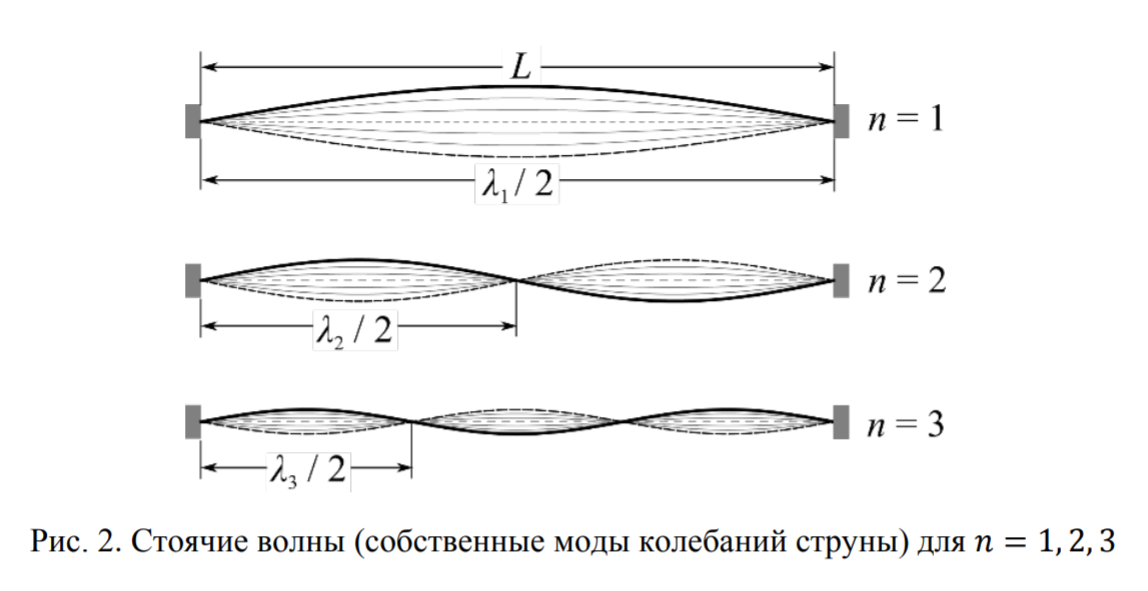
\includegraphics[width=\textwidth]{1.4.5 3}

При колебаниях реальной струны всегда имеет место потеря энергии
(часть теряется вследствие трения о воздух; другая часть уходит через неидеально закрепленные концы струны и т.д.). Поддержание незатухающих колебаний в струне может осуществляться точечным источником, в качестве которого в данной работе используется электромагнитный вибратор. При этом
возникает необходимость переноса энергии от источника по всей струне.

Рассмотрим вопрос о передаче энергии по струне. В стоячей волне поток
энергии вдоль струны отсутствует — колебательная энергия, заключенная
в отрезке струны между двумя соседними узлами, не транспортируется в другие части струны.Передача энергии между различными участками струны возможна
только благодаря бегущим волнам, которые, однако, в рассмотренной выше
идеальной модели струны не возникают. Парадокс снимается, если учесть,
что из-за потерь энергии при отражении волны от концов не происходит полной компенсации падающей и отраженной волны, поэтому к стоячей волне
на струне добавляется малая бегущая компонента — именно она служит «разносчиком» энергии по всей системе.

Для достижения максимального эффекта от вибратора, его следует располагать вблизи узловой точки, так как амлитуда $a = 2A sin(kx) \Rightarrow 2A = \frac{a}{sin(kx)}\rightarrow \infty$, но из-за нелинейных эффектов и сил трения амплитуда ограничивается некоторым значением.\\

\section{Экспериментальная установка}

\subsection{Схема установки}

Схема установки приведена на Рис. 3. Стальная гитарная струна 1 закрепляется в горизонтальном положении между двумя стойками с зажимами 2 и 3,
расположенными на массивной станине 4. Один конец струны закреплен в
зажиме 2 неподвижно. К противоположному концу струны, перекинутому через блок, прикреплена платформа с грузами 5, создающими натяжение
струны. Зажим 3 можно передвигать по станине, устанавливая требуемую
длину струны. Возбуждение и регистрация колебаний струны осуществляются с помощью электромагнитных датчиков (вибраторов), расположенных
на станине под струной. 

Электромагнитный датчик 6 подключен к звуковому
генератору 7 и служит для возбуждения колебаний струны, частота которых
измеряется с помощью частотомера 10 (в некоторых установках частотомер
встроен в генератор). 

Колебания струны регистрируются с помощью электромагнитного датчика 8, сигнал с которого передается на вход осциллографа 9.
Разъёмы, через которые датчики с помощью кабелей соединяются с генератором и осциллографом, расположены на корпусе станины.

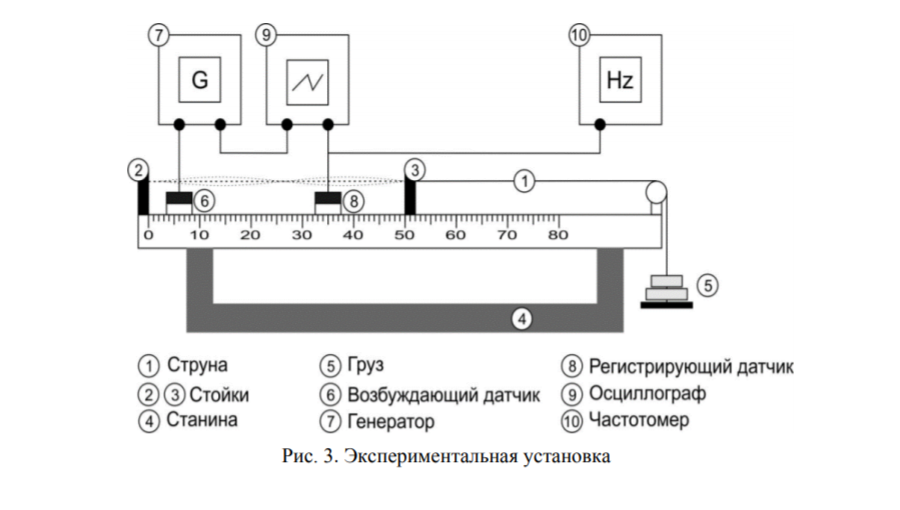
\includegraphics[width=\textwidth]{1.4.5 4}

\subsection{Принцип работы датчиков}

Устройство и внешний вид электромагнитного датчика показаны на Рис. 4.
В пластмассовом корпусе датчика закреплен подковообразный магнит. На полюсах
магнита намотаны соединенные последовательно катушки переменного тока, который подается с генератора. Магнитное
поле в зазоре между полюсами электромагнита складывается из поля постоянного
магнита $B_0$ и малой добавочной составляющей поля катушек $B_{\sim} \ll B_0$ . Сила, с которой электромагнит действует на стальную
(магнитную) струну, пропорциональна
квадрату индукции B суммарного поля в
зазоре электромагнита :

\[ F\propto (B_0+ B_{\sim})^2 \approx B_0^2 + 2B_0B_{\sim} .\]

Отсюда видно, что при $B_{\sim} \ll B_0$ сила $F$ линейно зависит от переменного
поля $B_{\sim}$, а значит и от тока в катушках (т. к. $B_{\sim}  \propto I_{\sim}$), и поэтому частота переменой силы $ F_{\sim} \propto I_{\sim}$, действующей на струну, совпадает с частотой генератора. То есть участок струны, расположенный над электромагнитом, совершает колебательное движение в вертикальной плоскости с частотой задающего генератора. Колебания далее передаются по всей струне и,
если частота колебаний совпадает с одной из собственных частот струны, на
струне устанавливается стоячая волна. 

\begin{center}
    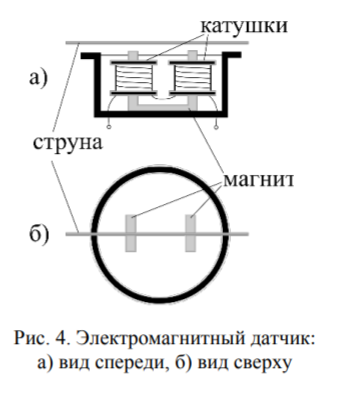
\includegraphics[scale=0.7]{1.4.5 5}
\end{center}

Колеблющаяся струна возбуждает в
регистрирующей катушке переменную ЭДС с амплитудой, пропорциональной амплитуде колебаний струны. Сигнал ЭДС измеряется с помощью осциллографа.
Отметим, что магнитное поле наиболее однородно по координате в центральной части электромагнита, поэтому датчики должны быть повернуты
так, чтобы струна располагалась в центральной части перпендикулярно к полюсам магнита. Возбуждающий датчик следует расположить вблизи неподвижного конца струны (ближе к узлу), а регистрирующий — в пучности.\\

\subsection{Измерения с помощью осциллографа}

Для регистрации колебаний струны в работе используется электронный
осциллограф, соединённый с электромагнитным датчиком 8. Он позволяет
регистрировать колебания в случаях, когда это невозможно сделать визуально. Также с помощью осциллографа можно измерять амплитуду возбуждения и форму сигнала, что даёт возможность установить, является ли режим
возбуждения стоячих волн линейным, иными словами, имеет ли место прямая пропорциональность между силой возбуждения и амплитудой колебаний
струны, и не возникает ли отклонений от закона. 

Контролировать величину и форму сигнала колебаний струны на экране
осциллографа можно несколькими способами: в одноканальном (переключатель $MODE$ в положении $CH2$) и двухканальном (переключатель $MODE$ в положении $DUAL$) режимах работы осциллографа — по временной развертке
сигналов, а также в режиме сложения двух взаимно перпендикулярных сигналов — основного и опорного (режим $X$--$Y$).

При возбуждении стоячей волны на экране осциллографа в режиме развертки должен появиться сигнал синусоидальной формы. При чрезмерном
возбуждении вид синусоиды искажается, что свидетельствует об отклонении
от линейного режима. В двухканальном режиме осциллографа можно сравнить опорный (подаваемый одновременно на возбудитель колебаний 6 и канал CH1 осциллографа) и основной (снимаемый с датчика 8) сигналы — в
отсутствие нелинейных искажений они должны совпадать. Кроме того, в режиме сложения сигналов ($X–Y$) на экране должен прорисовываться эллипс
правильной формы.

Дополнительным критерием того, что частота гармоники определена
верно, является симметричность «резонансной кривой» — амплитудно-частотной характеристики системы (Рис. 5). А именно, при подходе к резонансной частоте со стороны как высоких, так и со стороны низких частот, максимум сигнала наблюдается при одном и том же значении частоты.

\begin{center}
    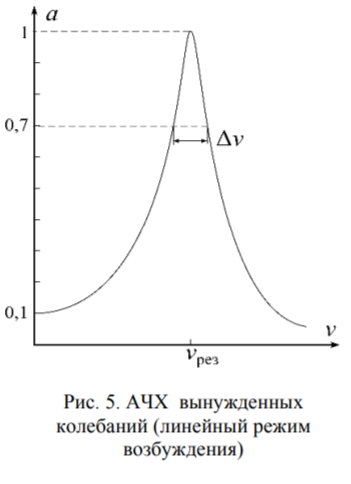
\includegraphics[width=9cm]{1.4.5 6}
\end{center}

\section{Ход работы}

\subsection{Установка грузов} 

Освобождаем зажим струны на стойке $3$, устанавливаем длину струны $L = 50$ см. Натягиваем струну, поставив на платформу грузы суммарной массой ($m_{\text{г}} \approx 0,985 $ кг), с учетом веса платформы и крепежа $m_{\text{пл}} \approx 0,113$ кг. Осторожно зажимаем струну в стойке, не деформируя струну. В свою очередь возбуждающий датчик $6$ должен располагаться рядом с неподвижной
стойкой $2$, вблизи узла стоячей волны.\\

\subsection{Предварительные расчеты}

Оценим скорость распространения волн с учётом того, что известная линейная плотность струны $\rho_l = 568,4 \cdot 10^{-6} \text{кг/м}$:
\[u = \sqrt{\frac{(m_{\text{пл}} + m_{\text{г}})g}{\rho_l}} \approx 137,7\text{ м/с}\]

Частота основной гармоники равна 
\[\nu_1 = \frac{u}{\lambda_1} = \frac{u}{2L} = 137,7 \text{ Гц}\]

\subsection{Визуальное наблюдение}

Включим в сеть звуковой генератор (частотометр встроен в генератор). Установим на генераторе тип сигнала — синусоидальный, частоту основной гармоники $\nu_1$ и
максимальную амплитуду напряжения -- $20$ В. При этом сигнал с выхода генератора подадим на возбуждающий датчик.

Медленно меняя частоту звукового генератора в диапазоне $\nu = \nu_1 \pm 5 \text{ Гц}$ стараемся добиться возбуждения стоячей волны на основной гармонике (одна пучность). Видно, что даже на максимальной амплитуде визуально колебания наблюдать невозможно, также понятно, что струна не может касаться датчика на заданной амплитуде.

Настраиваем осциллограф нужным образом и переходим к следующей части.\\

\subsection{Регистрация стоячих волн с помощью осциллографа}

Установим регистрирующий датчик в центре под струной (в пучности стоячей волны). Проверяем правильность соединения проводов. Сигнал колебаний струны с регистрирующего датчика $8$ (основной сигнал) подается на вход канала $CH2(Y)$ осциллографа. На вход канала $CH1(X)$ подается опорный сигнал с генератора на
частоте возбуждения струны.

Включим осциллограф в сеть. Для наблюдения колебаний струны в одноканальном режиме переключатель режима работы $MODE$ блока вертикального отклонения ставим в положение $CH2$; тумблер режима работы канала $Y$ — в положение $AC$;
на блоке синхронизации устанавливаем $SOURCE$ — $CH2$. Установим такие значения коэффициента усиления канала $Y (VOLTS/DIV)$; постоянную времени
развертки ($TIME/DIV$) и уровень синхронизации $(LEVEL)$, чтобы на экране
было удобно наблюдать форму сигнала.

\subsection{Таблицы полученных данных}

Для дальнейших измерений силы натяжения будем использовать формулу \[ T = (m_{\text{пл}} + m_{\text{г}})g.\]

Где $m_{\text{пл}}$ -- масса установки (платформы и крючка), а $m_{\text{г}}$ -- масса подвешенных грузиков, которую мы изменяем на протяжении эксперимента.

Для нечётных гармоник регистрирующий датчик расположим посередине струны, так как там всегда находится пучность. Для нечётных гармоник подберём следующие расстояния от возбуждающего датчика в областях пучности, чтобы было удобно расположить регистрирующий датчик:
\[l_2 = (1\cdot\frac{50}{2} +  \frac{1}{2}\frac{50}{2})\text{ см} = 37,5\text{ см}\] 
\[l_4 = (2\cdot\frac{50}{4} +  \frac{1}{2}\frac{50}{4})\text{ см} = 31,5\text{ см}\] 
\[l_6 = (3\cdot\frac{50}{6} +  \frac{1}{2}\frac{50}{6})\text{ см} = 29,17\text{ см}\] 
\[l_8 = (4\cdot\frac{50}{8} +  \frac{1}{2}\frac{50}{8})\text{ см} = 28,125\text{ см}\] 
\[l_{10} = (5\cdot\frac{50}{10} +  \frac{1}{2}\frac{50}{10})\text{ см} = 27,5\text{ см}\] 

Для каждого натяжение будем считать теоретическое значение частоты основной гармоники, чтобы потом по нему подбирать резонансную частоту. Снимаем данные и заносим их в таблицы:

\begin{center}
\begin{tabular}{|c|c|c|c|c|c|c|c|c|c|c|}
\hline 
\multicolumn{11}{|c|}{$\textbf{Натяжение } T_1 = 10,98H, \text{ } \nu_{\text{теор}} = 137,7 \text{ Гц}$} \\ 
\hline 
$n$ & $1$ & $2$ & $3$ & $4$ & $5$ & $6$ & $7$ & $8$ & $9$ & $10$ \\ 
\hline 
$\nu_n$, Гц & $137$ & $276$ & $417$ & $557$ & $697$ & $838$ & $982$ & $1125$ & $1267$& $1408$\\
\hline
\end{tabular} 
\end{center}

\begin{center}
\begin{tabular}{|c|c|c|c|c|c|c|c|c|c|c|}
\hline 
\multicolumn{11}{|c|}{$\textbf{Натяжение } T_2 = 14,41H, \text{ } \nu_{\text{теор}} = 159,2 \text{ Гц}$} \\ 
\hline 
$n$ & $1$ & $2$ & $3$ & $4$ & $5$ & $6$ & $7$ & $8$ & $9$ & $10$ \\ 
\hline 
$\nu_n$, Гц & $158$ & $318$ & $478$ & $641$ & $799$ & $963$ & $1122$ & $1279$ & $1422$& $1603$\\
\hline
\end{tabular} 
\end{center}

\begin{center}
\begin{tabular}{|c|c|c|c|c|c|c|c|c|c|c|}
\hline 
\multicolumn{11}{|c|}{$\textbf{Натяжение } T_3 = 19,65H, \text{ } \nu_{\text{теор}} = 186 \text{ Гц}$} \\ 
\hline 
$n$ & $1$ & $2$ & $3$ & $4$ & $5$ & $6$ & $7$ & $8$ & $9$ & $10$ \\ 
\hline 
$\nu_n$, Гц & $185$ & $369$ & $557$ & $742$ & $930$ & $1116$ & $1303$ & $1491$ & $1680$& $1868$\\
\hline
\end{tabular} 
\end{center}

\begin{center}
\begin{tabular}{|c|c|c|c|c|c|c|c|c|c|c|}
\hline 
\multicolumn{11}{|c|}{$\textbf{Натяжение } T_4 = 24,48H, \text{ } \nu_{\text{теор}} = 207,5 \text{ Гц}$} \\ 
\hline 
$n$ & $1$ & $2$ & $3$ & $4$ & $5$ & $6$ & $7$ & $8$ & $9$ & $10$ \\ 
\hline 
$\nu_n$, Гц & $205$ & $411$ & $618$ & $823$ & $1032$ & $1236$ & $1445$ & $1651$ & $1863$& $2067$\\
\hline
\end{tabular} 
\end{center}

\begin{center}
\begin{tabular}{|c|c|c|c|c|c|c|c|c|c|c|}
\hline 
\multicolumn{11}{|c|}{$\textbf{Натяжение } T_5 = 29,39H, \text{ } \nu_{\text{теор}} = 227,4 \text{ Гц}$} \\ 
\hline 
$n$ & $1$ & $2$ & $3$ & $4$ & $5$ & $6$ & $7$ & $8$ & $9$ & $10$ \\ 
\hline 
$\nu_n$, Гц & $224$ & $450$ & $675$ & $902$ & $1127$ & $1352$ & $1580$ & $1807$ & $2034$& $2262$\\
\hline
\end{tabular} 
\end{center}

\subsection{Обработка результатов измерений №1.\\ Сравнение значений частот}

Полученные значения очень близки к теоретическим, потому что законы, описывающие поведение струны, очень точны, а так же погрешность измерений крайне мала ввиду высокой точности осциллографа, генератора частот.

Благодаря высокой добротности струны, возможно возбуждение её
колебаний при кратных частотах генератора, меньших, чем $\nu_1$. Для наблюдения явления переключаем осциллограф в режим ($X$--$Y$) и настраиваем установку
на наблюдение основной гармоники. Затем уменьшаем частоту возбуждения
в два раза, установив на генераторе $\nu$ = $\nu_1/2$. На экране осциллографа должна
наблюдаться фигура Лиссажу с одним самопересечением. Приведём снятую фотографию фигуры:

\begin{center}
    \includegraphics[width=13cm]{1.4.5 11}
\end{center}

\subsection{Определение добротности $Q$ струны как колебательной системы}

Измерив её амплитудно-частотную характеристику (АЧХ) вблизи одной из резонансных частот (в качестве таковых выбрана $\nu_1$).

Для расчётов воспользуемся известным из теории колебаний результатом:
добротность колебательной системы связана с резонансной частотой $\nu_{\textbf{рез}}$ и шириной резонансной кривой $\bigtriangleup \nu$ соотношением \[ Q = \frac{\nu_{\textbf{рез}}}{\bigtriangleup \nu} , \]
где ширина резонансной кривой $\bigtriangleup \nu$ измеряется на уровне амплитуды, составляющей $0,7$ от амплитуды в резонансе
(Рис. 5).

\begin{center}
    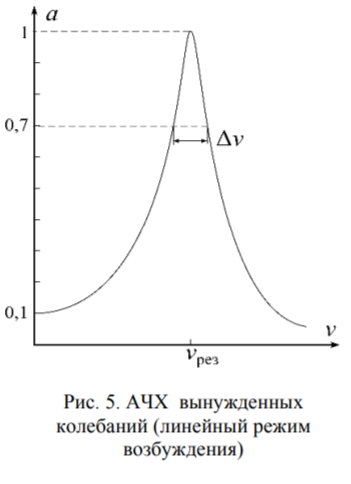
\includegraphics[width=7cm]{1.4.5 6}
\end{center}

По формуле получим оценку добротности $Q$ струны как колебательной системы: $Q \approx \frac{\nu_{\textbf{рез}}}{\bigtriangleup \nu} = \frac{223 \text{Гц}}{0,12 \text{Гц}} \approx 1860$\\

Заметим, что найти добротность колебаний струны более точным способом с помощью графика не получилось, так как при заданной резонансной частоте происходит медленные колебания амплитуды напряжения на осциллографе из-за малой компоненты бегущей волны (она всегда присутствует в сточей волне из-за коэффициента отражения от краёв струны), поэтому мы ограничились лишь оценкой величины добротности.

\newpage

\subsection{Обработка результатов измерений №2}

Графики зависимости $\nu_n(n)$ для различных $T$:

\begin{center}
    \includegraphics[width = 13cm]{1.4.5 9}
\end{center}

Найдём коэффициенты для зависимости через метод наименьших квадратов:
\[\frac{u}{2L} = \frac{\langle \nu^2_n \rangle}{\langle \nu_n n \rangle}\]
\[\Delta(\frac{u}{2L}) = \sqrt{\frac{1}{9}\Big( \frac{\langle \nu^2_n \rangle}{\langle n^2 \rangle} - \Big(\frac{u}{2L}\Big)^2\Big)} = \frac{\Delta u}{2L} - \frac{\Delta L u}{2L^2} \Rightarrow\]
\[\Rightarrow \Delta u = 2L 
\Big( \sqrt{\frac{1}{9}\Big( \frac{\langle \nu^2_n \rangle}{\langle n^2 \rangle} - \Big(\frac{u}{2L}\Big)^2\Big)} + \frac{\Delta L u}{2L^2}\Big)\]

Здесь $\Delta L$ -- погрешность определения расстояния при установке длины струны. Положим её равной $0,1$ см.
 
Построим таблицу расчитанных значений скоростей волн и погрешностей:
\begin{center}

\begin{tabular}{|c|c|c|c|}
\hline 
$T$, H & $u\textbf{,} \frac{\textbf{м}}{\textbf{с}}$ & $\Delta u\textbf{,} \frac{\textbf{м}}{\textbf{с}}$ & $\varepsilon_{u}, \% $ \\ 
\hline 
$10,98$ & 140,38 & 0,73 & 0,52 \\ 
\hline 
$14,41$ & 159,74 & 0,70 & 0,44 \\ 
\hline 
$19,65$ & 186,42 & 1,09 & 0,58 \\ 
\hline 
$24,48$ & 206,42 & 0,94 & 0,46 \\ 
\hline 
$29,39$ & 226,41 & 0,99 & 0,49 \\ 
\hline 
\end{tabular}
\end{center} 
\[ \]

{\bf Обработка результатов измерений $3$. Построение графика зависимости квадрата скорости $u^2$ от силы натяжения
$T$}

Построим таблицу $u^2(T)$, построим график полученной зависимости и определим погонную плотность струны $\rho_l$ и оценим погрешность результата. И в заключение сравним полученное значение со значением, указанным на установке.

Для погрешностей имеем:
\[\Delta (u^2) = 2u\Delta u\]

\begin{center}
\begin{tabular}{|c|c|c|}
\hline 
$u^2$, м$^2$/c$^2$ & $\Delta (u^2)$, м$^2$/c$^2$& $T$, Н \\ 
\hline 
19706,54 &204,95& 10,98 \\ 
\hline 
25516,87 &223,636& 14,41 \\ 
\hline 
34752,42 &395,21& 19,65 \\ 
\hline 
42609,22 &388,07& 24,48 \\ 
\hline 
51261,49 &448,29& 29,39 \\ 
\hline 
\end{tabular} 
\end{center}

Так как известны погрешности значений $\Delta (u^2)$, найдём коэффициент наклона с помощью метода Пирсона (хи-квадрат):
\[\frac{1}{\rho_l} = \frac{\langle \frac{u^4}{(\Delta u^2)^2} \rangle}{\langle \frac{u^2 T}{(\Delta u^2)^2} \rangle}  = 1753,97 \text{ м/кг}\]
\[\rho_l = 570,1 \cdot 10^{-6} \text{ кг/м}\]
\[\Delta (\frac{1}{\rho_l}) = \frac{\Delta \rho_l}{\rho^2_l} = \sqrt{\frac{1}{4} \Big( \frac{\langle \frac{u^4}{(\Delta u^2)^2} \rangle}{\langle \frac{T^2}{(\Delta u^2)^2} \rangle}  - \frac{1}{\rho_l^2}\Big)} = 8,08 \text{ кг/м}\]
\[\Delta \rho_l = 2,63  \cdot 10^{-6} \text{ кг/м}\]

Строим график для подтверждения линейности зависимости:

\begin{center}
    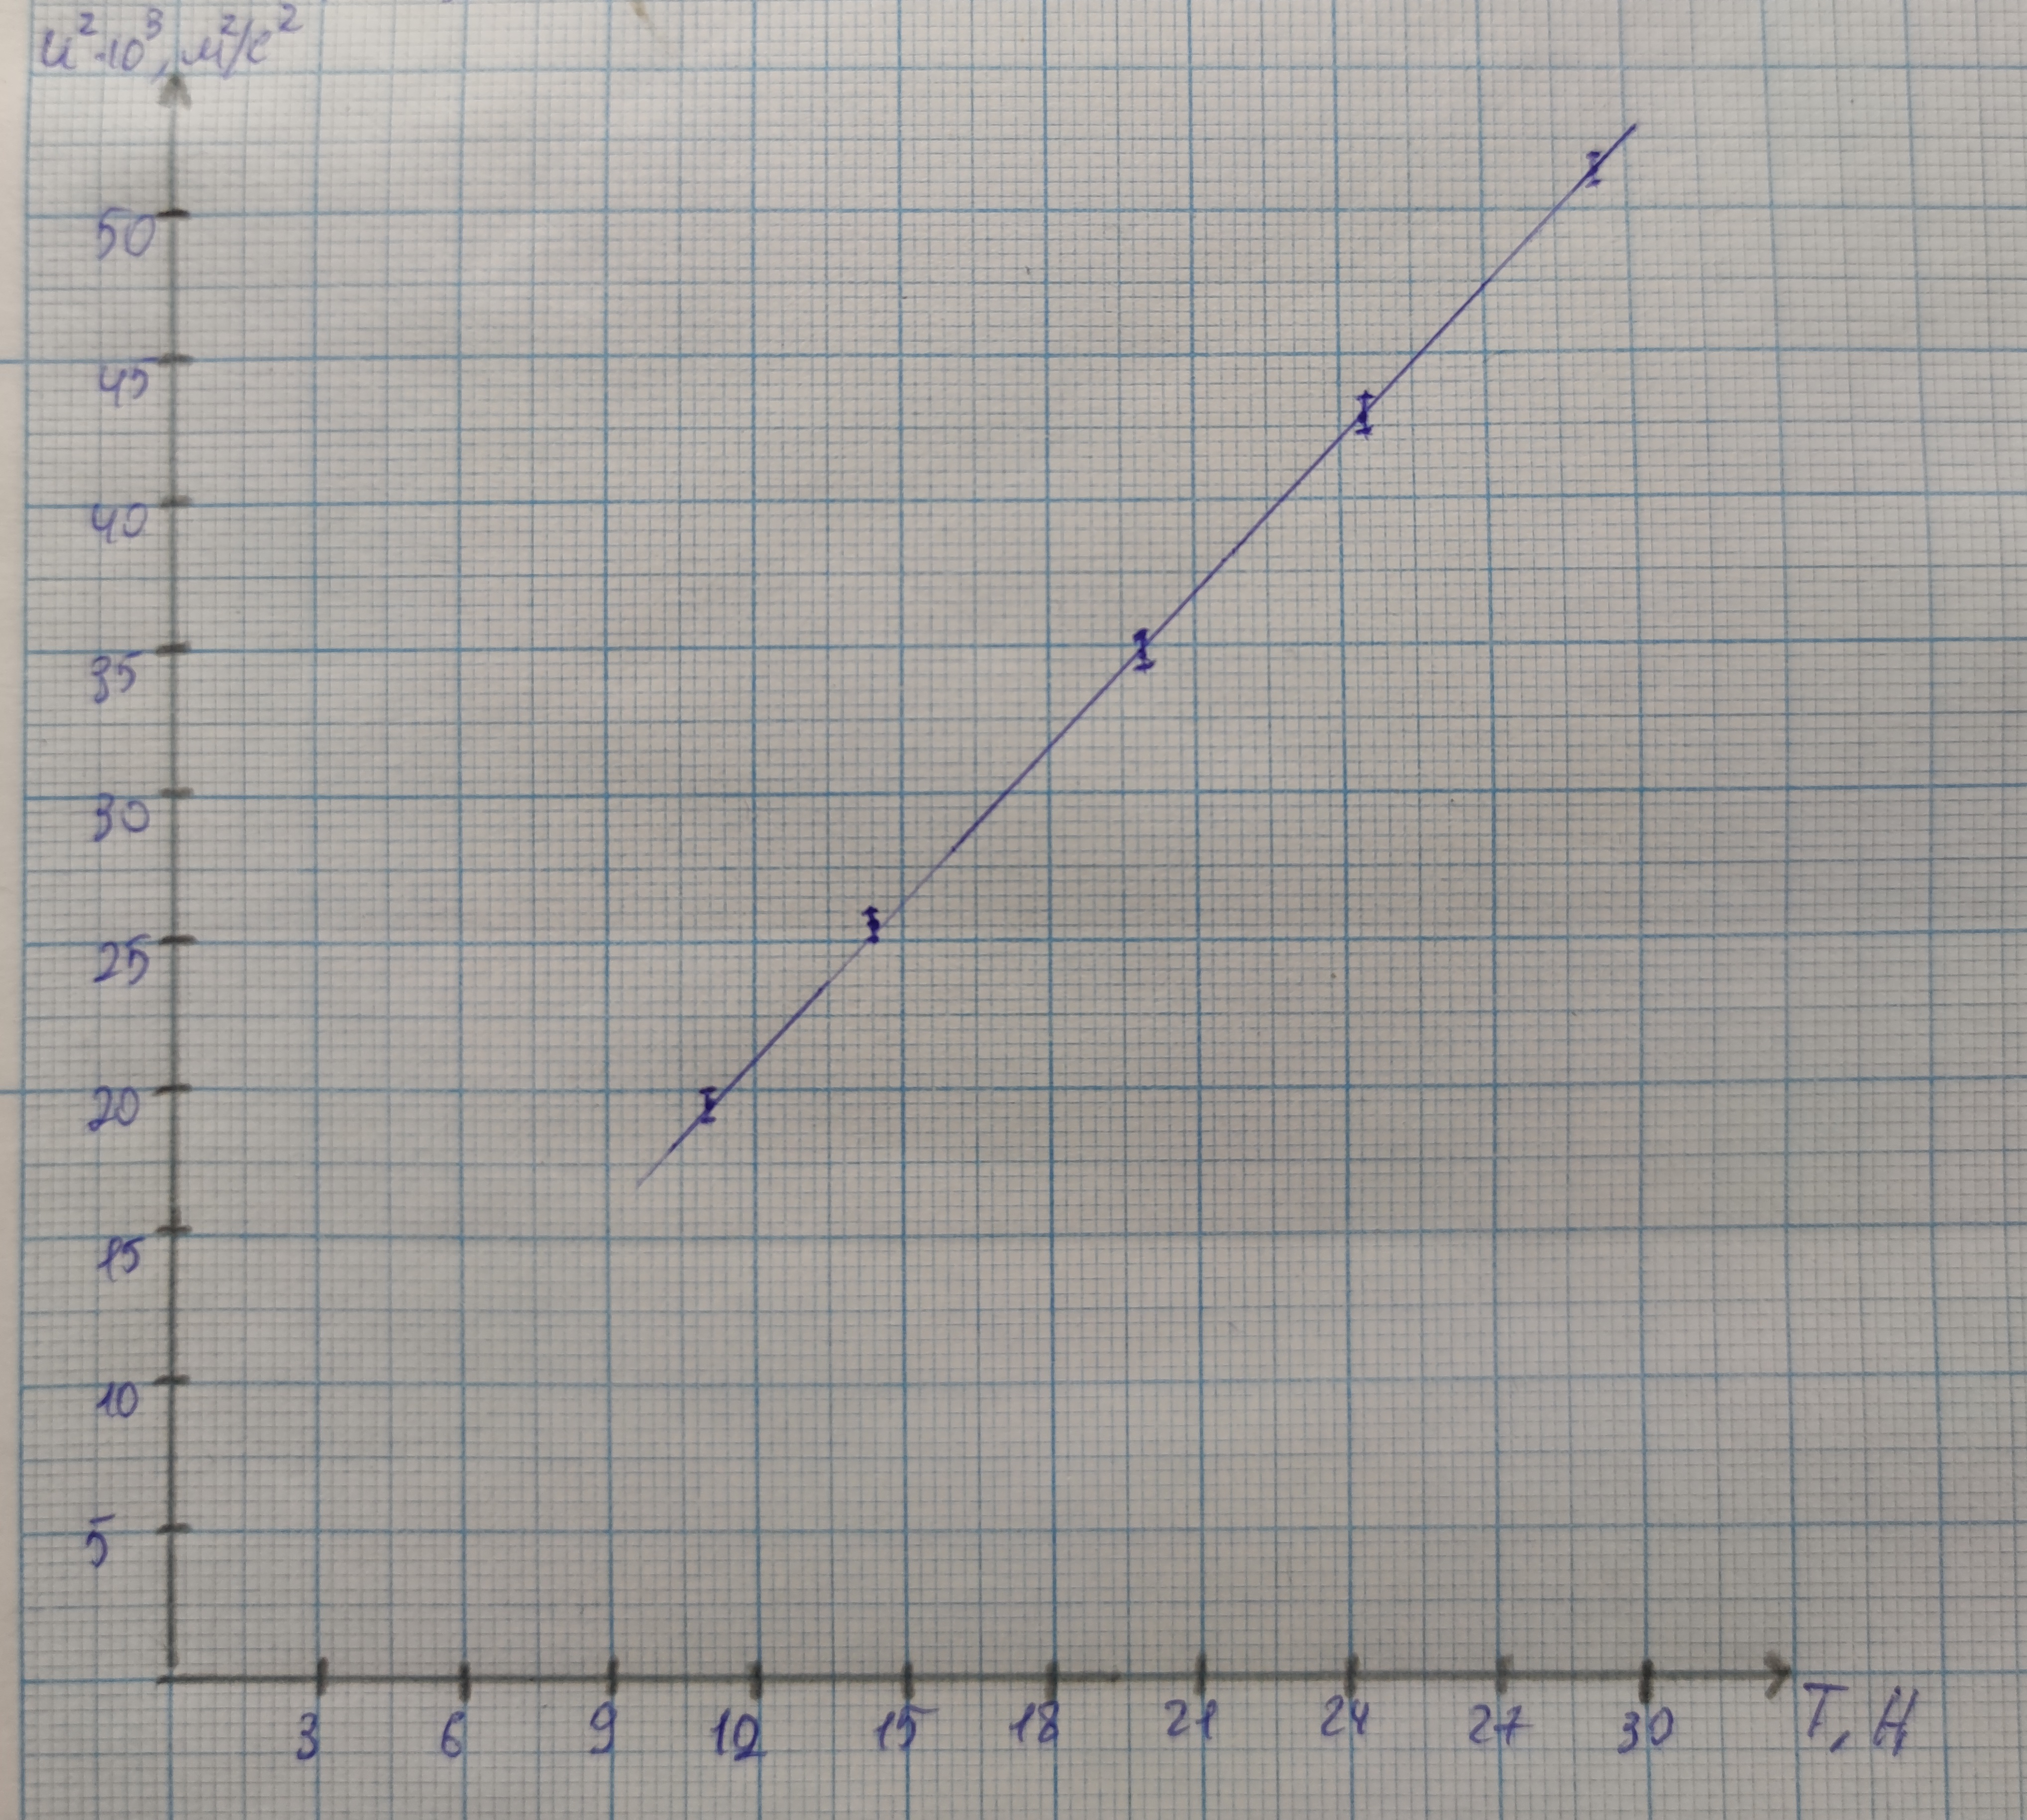
\includegraphics[width = 12cm]{1.4.5 10}
\end{center}

\section{Вывод}

Экспериментальным путем изучили поперечные стоячие волны на струне, научились определять собственные частоты колебаний струны, исследовали зависимость скорости распространения поперечных волн на струне в зависимости от ее натяжения. 

Экспериментальным путем нашли линейную плотность струны, которая практически совпадает со значением, указанным на установке: $\rho_l = 568,4 \cdot 10^{-6} \text{кг/м}$ с погрешностью, большей модуля разности экспериментального и теоретичекого значений.

\end{document}